\documentclass{beamer}

\usetheme{default}
\usecolortheme{crane}
\title{Presentation}
\subtitle{EE2227- Control Systems}
\usepackage{graphicx}
\graphicspath{{./images/}}

\author{
Md.Sadiq -  \
\texttt{EE18BTECH11051}
}
\institute{IIT HYDERABAD}
\date{February 10, 2020}

\subject{GATE Paper question solution}

\AtBeginSubsection[]
{
  \begin{frame}<beamer>{Outline}
    \tableofcontents[currentsection,currentsubsection]
  \end{frame}
}

\begin{document}

\begin{frame}
  \titlepage
\end{frame}

\begin{frame}{Outline}
  \tableofcontents
\end{frame}

\section{Problem Statement}

\begin{frame}{GATE EC 2015 Question}
 
 
   Q.The polar plot for the transfer function $ G(s) = \frac{10(s+1)}{10+s}$ for \\0 $\leq \omega < \infty$ will be in the \\
  (A) first quadrant\\
  (B) second quadrant\\
  (C) third quadrant\\
  (D) fourth quadrant\\
\end{frame}

\section{Polar Plot}

\begin{frame}{Polar Plot}

\begin{centre}

    The Polar plot is a plot, which can be drawn between the magnitude and the phase angle of $G(j\omega)H(j\omega)$ by varying $\omega$ from 0 to $\infty$. The polar graph sheet is shown in the following figure.
    \begin{figure}[!h]
    \centering
    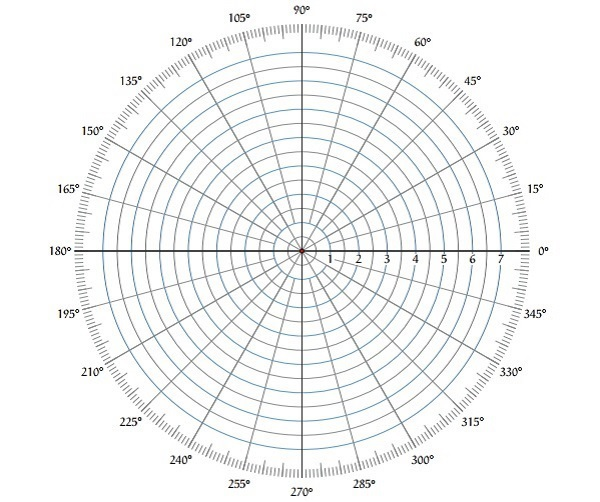
\includegraphics[width=\columnwidth]{./figs/ee18btech11051_fig1.png}
    \caption{Polar Plot}
    \label{fig:ee18btech11051_fig1}
    \end{figure}
\end{centre}



\end{frame}

\section{Solution}

\begin{frame}{Solution}
Substituting s = $j \omega$ in the given transfer function gives \\~\\
G(j$\omega$) = $\frac{10(1+j\omega)}{(10+j\omega)}$\\~\\
Here, taking 1 + j$\omega$ = $\sqrt{1+{\omega}^2}e^{j\tan^{-1}(\omega)}$,
\\~\\ and 10 + j$\omega$ = $\sqrt{10^{2}+{\omega}^2}e^{j\tan^{-1}(\frac{\omega}{10})}$,\\~\\
G(j\omega) = 10\sqrt{\frac{1+\omega^2}{100+\omega^2}}e^{j(\tan^{-1}(\omega)-\tan^{-1}(\frac{\omega}{10}))}
 

\end{frame}

\begin{frame}{Solution}
As 0 $\leq \omega < \infty$,\\~\\ 0 $\leq \tan^{-1}(\omega), \tan^{-1}(\frac{\omega}{10}) < \frac{\pi}{2}$;\\~\\
And as $\tan^{-1}$(x) is a monotonically increasing function,\\~\\

[ $\frac{d}{dx}\tan^{-1}(x)$ = $\frac{1}{1+x^2} >$  0  ]\\~\\
$\tan^{-1}(\omega) \geq \tan^{-1}(\frac{\omega}{10}) $, with equality as $\omega \rightarrow \infty$\\~\\
So, $|G(j\omega)| > 0 $ and $0 \leq \angle G(j\omega) < \frac{\pi}{2}$
\\~\\ Therefore, the polar plot of G(s) lies in the first quadrant. \\~\\ The plot of G(s) is:


\end{frame}

\section{Verification}


\begin{frame}{Plot of G(s)}
\begin{center}
      \begin{figure}[!h]
      \centering
      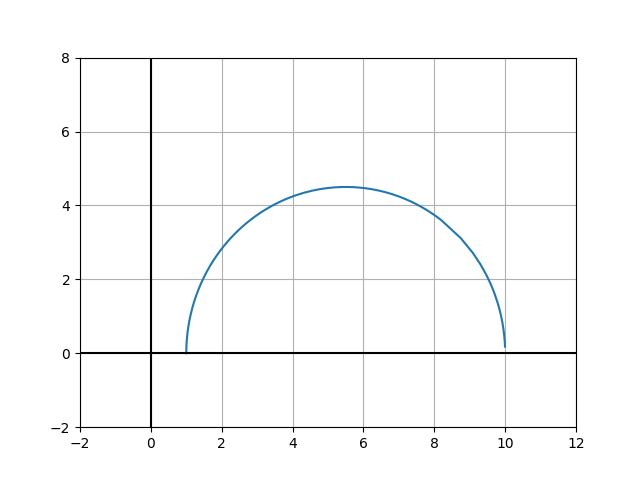
\includegraphics[width=\columnwidth]{./figs/ee18btech11051_fig2.png}
      \caption{Plot}
      \label{fig:ee18btech11051_fig2}
      \end{figure}
\end{center}

\end{frame}

\begin{frame}{Final Slide}
\begin{center}
    THANK YOU
\end{center}
    
\end{frame}
    

\end{document}

